\chapter{State of the Art\label{cha:chapter2}}

\section{Object Detection Methods}
State of the art object detection methods include \textit{scale invariant feature transformation} (SIFT) \cite{Lowe2004DistinctiveKeypoints}, \textit{speeded up robust features} (SURF) \cite{Bay2008Speeded-UpSURF}, \textit{binary robust invariant scalable
keypoints} (BRISK) \cite{Leutenegger2011BRISK:Keypoints}, \textit{oriented fast and rotated BRIEF} (ORB) \cite{Rublee2011ORB:SURF}, \textit{Accelerated KAZE} (AKAZE, KAZE meaning wind in Japanese) \cite{Alcantarilla2012KAZEFeatures, Alcantarilla2013FastSpaces} and \textit{template matching} (TM) \cite{Brunelli2009TemplatePractice}. The two latter shall be discussed here briefly.\newline

AKAZE feature matching is a pyramidal object detection algorithm. The Pyramidal approach declines the image ratio with every filtering step. Spanning over several scales features are detected and described. In contrast to other established algorithms like SIFT, which use a linear scale space for filtering, AKAZE instead uses a nonlinear scale space with the recently developed numerical model \textit{Fast Explicit Diffusion}. The advantage of the nonlinear scale space is depicted in figure  \ref{skalenraum}. Prominent features like edges and corners are preserved. 
\begin{figure}[ht]
	\centering
  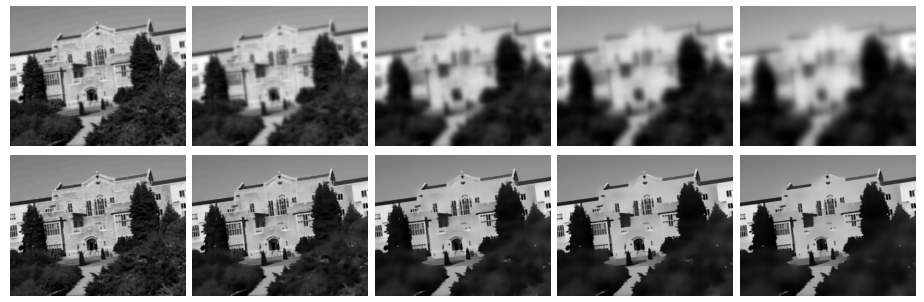
\includegraphics[width=\textwidth]{nonlinearscalespace.png}
	\caption{Top row: Gauss filtering with linear scale space and increasing standard deviation. Bottom Row: Non linear diffusion scale space. \cite{Alcantarilla2012KAZEFeatures}}
	\label{skalenraum}
\end{figure}
The outcome of AKAZE is depicted in fig \ref{AKAZE}. Matches are shown as dots connected with lines between the two pictures of the same object from another point of view.
\begin{figure}[ht]
	\centering
  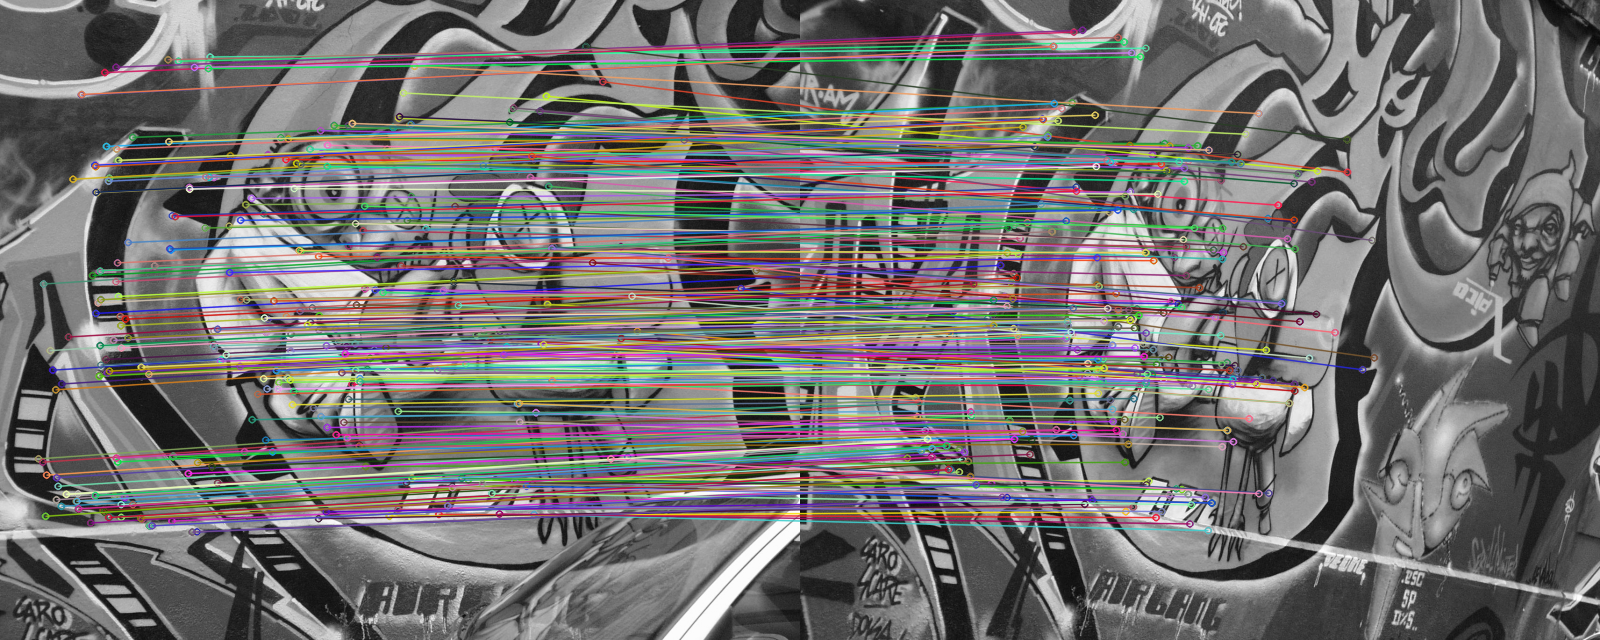
\includegraphics[width=\textwidth]{AKAZE.png}
	\caption{AKAZE Feature Matching for a grafitti viewed from two different angles. Best viewed in color. \cite{Documentation.LastVisited2018-11-15.TutorialMatching}}
	\label{AKAZE}
\end{figure}
 \newline
TM unlike AKAZE matches templates instead of features. Fig \ref{templatematching} illustrates this process. In the left image the face of the man is to be found. The template is the little cut-out in the middle. Pixel by pixel the template is being convoluted with the original image and rated with a metric. The resulting resolution matrix is depicted on the right. Bright areas indicate potential findings. At the brightest point the template is rightfully suggested.

\begin{figure}[ht]
	\centering
  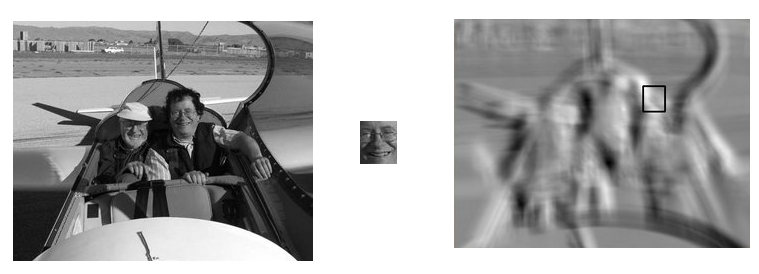
\includegraphics[width=\textwidth]{templatematching.png}
	\caption{In the picture on the left the template in the middle is to be found. Depicted on the right is the resolution matrix with potential findings indicated with the bright color and the found area of the template in the original image.\cite{Documentation.LastVisited2018-11-15.2014TemplateMatching}}
	\label{templatematching}
\end{figure}

\section {Service Interfaces}
\label{serviceinterfaces}
In this section potential client-server-based interfaces and underlying protocols for the object detection service shall be discussed. The evaluated interfaces are \textit{Advanced Message Queuing Protocol} (AMQP), \textit{message queuing telemetry transport} (MQTT), \textit{representational state transfer} (REST), \textit{Google remote procedure calls} (gRPC), \textit{graph query language} (GraphQL) and \textit{open platform communication unified architecture vision} (OPC UA Vision). \newline

Both AMQP 0.x and MQTT are broker based protocols. They are protocols specialized for machine-to-machine (M2M) communication. Clients can be sensors, programmable logic controllers etc., the server is a broker connecting the clients. A broker is a central instance mediating between parties. Clients can subscribe to various message queues called topics. Telemetry data can then be published and read from these topics handled by the broker. The clients dynamically change between publisher and subscriber. Fig \ref{MQTT} illustrates the MQTT architecture.  \cite{Banks2014MQTT3.1.1} RabbitMQ is a message broker software which supports AMQP 0.x natively and MQTT via a plugin. \cite{Lastvisited2018-15-122018WhichSupport} AMQP needs to be distinguished between 0.x and 1.0, as the underlying messaging paradigm has been completely revised. While for version 0.x strict publishing/subcription messaging is required, version 1.0 is based on a peer-to-peer connection where a broker is not required, although possible. Due to the more complex version of version 1.0, fewer implementations exist. \cite{Dizdarevic2018SurveyIntegration}

\begin{figure}[ht]
	\centering
  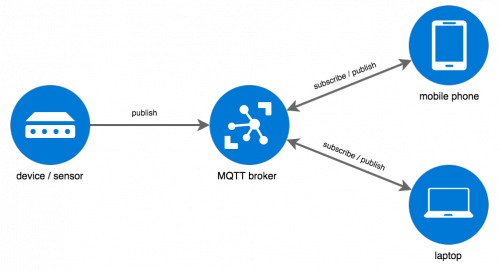
\includegraphics[width=0.9\textwidth]{MQTT.png}
	\caption{MQTT Architecture with the broker in the middle as a mediator between the clients.\cite{2018-11-24Pure-javascript-MQTT-broker}}
	\label{MQTT}
\end{figure}

REST is an architectural paradigm describing how distributed systems can communicate with each other. It consists of five mandatory and one optional restriction. If any of the five mandatory restrictions are violated, an architecture cannot be RESTful. The restrictions are 
\begin{enumerate}
    \item Client–server architecture
    \item Statelessness
    \item Cacheability
    \item Layered system
    \item Uniform interface
    \item Code on demand (optional)
\end{enumerate}
REST was developed by Roy Fielding alongside to HTTP/1.1 and although is not dependent on it, is the primary used protocol to implement REST. Thus, many web pages fulfill these restrictions naturally. REST messages are usually human readable JSON files. Unlike MQTT, REST does not rely on a broker.  \cite{Fielding2000ArchitecturalArchitectures} \newline

For many cases in the past it was hard for the maintainers to adhere to all REST principles due to its strict nature. Moreover, REST is usually implemented with HTTP/1.1. In 2015 HTTP/2 was released to adress the flaws of its predecessor. \cite{SayfanLastvisited2018-11-242018RESTAPIs} Among those are the lack of ability of constant data streaming, latency issues etc. gRPC fully takes advantage of HTTP/2 and thus has some advantage over REST. It uses stubs to describe an interface. Stubs are independent of any programming language. Unlike in most implementations of REST, gRPC does not use textual transport data like JSON but relies on Protobuf, a binary buffer. Moreover, Google offers an \textit{Extensible Server Proxy} (ESP), which offers a transcoding from HTTP/JSON to gRPC. \cite{2018-11-242017Grpc-gateway, Lastvisited2018-11-272018CloudGRPC} \newline

\begin{figure}[ht]
	\centering
  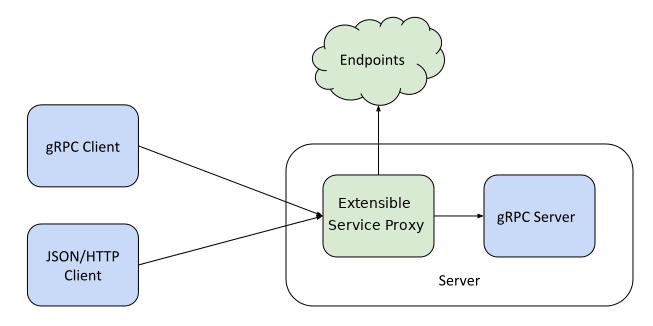
\includegraphics[width=0.7\textwidth]{gRPC_ESP.png}
	\caption{Deployed endpoints gRPC application. \cite{Lastvisited2018-11-272018CloudGRPC}}
	\label{ESP}
\end{figure}

GraphQL is a data query and -manipulation language. It was developed by Facebook and is open source since 2015. Compared to REST it is has a more flexible and efficient approach. Increase in efficiency over REST is based on faster mobile data access, and more flexibility for the API to let clients access precisely the data it needs,  i.e. the server modifies the data with respect to the clients needs instead of providing one rigid resource. \cite{LastVisited2018-15-122018BasicsIntroduction} 

OPC UA Vision is a companion specification adressing robotics and object detection. \cite{VDMA2018OPCSpecification} It's scope is to standardize the interfaces between the machine vision system and its process environments. A possible use case would be a conveyor belt that should be halted if any higher system level tells it to do so. Then, image acquisition can conducted by the machine vision system. As soon as image acquisition is done, an event should be fired which tells the higher production system the result of the acquisition. The conveyor belt can then continue. In June 2018 the first part of OPC UA Vision was released. This parts includes the basic skills on the infrastructure layer, such as result transmission, machine status etc. The following parts which have not been released yet should include machine vision skills such as post detection or a completeness check. As of now, there is no implementation of OPC UA Vision available and thus can only be used on an conceptual level.

\section {Deployment Options}
\label{deploymentoptions}
In the last decade, most applications had a monolithic character which did not focus much on scalability and interfaces. With the progress in digitalization, applications had to become more flexible and faster. To address this problem, the container architecture came about. Unlike a virtual machine which needs an operating system, runtime, system variables etc. to operate well, docker and others are sandbox systems which can imply all the mentioned features and furthermore can run on almost any operating system. See figure \ref{container} for an illustration. In the following, two possible deployment options are discussed, namely Heroku and Docker.\cite{WurbsLastvisited2018-11-272017DockerVeraendern}

\begin{figure}[ht]
	\centering
  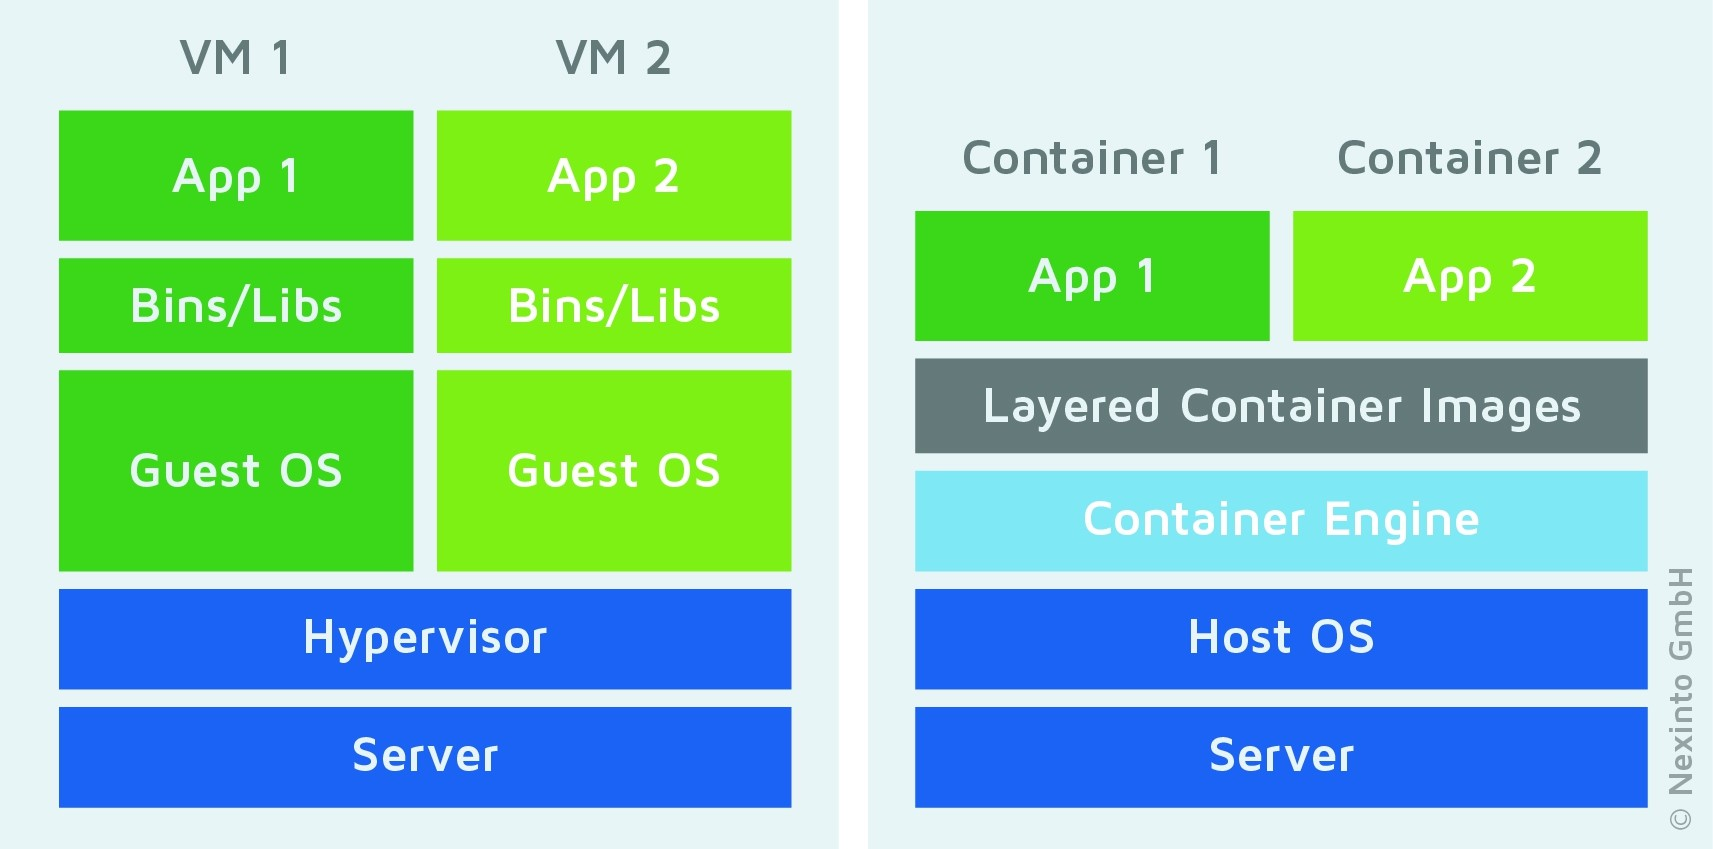
\includegraphics[width=0.7\textwidth]{containervsvm.jpg}
	\caption{Virtual machine architecture on the left versus container architecture on the right. Docker does not rely on a hypervisor.\cite{WurbsLastvisited2018-11-272017DockerVeraendern}}
	\label{container}
\end{figure}

Docker is an open source standard for operating-system-level virtualization. If docker is installed on an operating system, it is possible to run several apps on the machine simultaniously, with low start and stop times and little overhead. In combination with a continuous integration and continuous delivery platform, development and operations can be harmonized.

Heroku is a platform as a service provider which underlying technology shares some core concepts with Docker. E.g. BuildPacks are a set of scripts which are used to setup the final state of an image. The pendant on the Docker side is called Dockerfile. See \cite{ThurigLastvisited2018-27-112014DockerHeroku} for a full description of the similarities and \ref{dockerandheroku} for a list of pendants. However, there are also differences for the two alternatives. The main one is the dependency on the Heroku platform on the Heroku side, whereby on the Docker side one is completely flexible to choose any environment from Raspberry Pi to cloud platform providers like Amazon Web Services. This also means a surplus of workload on infrastructure on the Docker side. Also, one is less flexible on the prices. Heroku has a staged price model ranging from 0 to 500\,\$ per month and dyno. Docker is again more flexible in letting one just paying for the hosting and storaging and leaving the additional features provided by Heroku aside. \cite{ChrisLastvisited2018-11-272017WhyDocker} 


\begin{table}
\begin{center}
      \caption{Similar core concepts of Docker and Heroku. \cite{ThurigLastvisited2018-27-112014DockerHeroku}}
  \begin{tabular}{ l | l }
    Docker & Heroku  \\ \hline
Dockerfile &	BuildPack \\ 
Image	& Slug\\ 
Container&	Dyno\\ 
Index	&Add-Ons\\ 
CLI	&CLI
  \end{tabular}
  \label{dockerandheroku}
\end{center}
\end{table}

\section{Service Oriented Architectures}
Industrial Image Processing Applications as Orchestration of Web Services
\section{Communication between Object Detection System and Client}
If two humans want to communicate with one another, they need matching channels and they need to speak the same language. A channel is a mean of transport for information, e.g. sign language, smoke signs, mobile phones etc. If one entity tries to call someone via phone if the other does not have a phone, the caller enters the wrong number, the other has its phone turned off, they cannot communicate. In case they both have a phone, the called entity answers and both speak a common language (e.g. English), exchange of information can be achieved. Communication within technical systems faces the same challenges. As for the right channel, models like the OSI basic reference model for information technology standardized by ISO layer the transfer of information from the physical layer consisting of peaks in currents and voltages up until the application layer which includes direct user interaction, resource availability and so forth. \cite{InternationalOrganizationForStandardization1996ISO/IECEd.} This model and the protocols adhering to it ensure that information is delivered safely between communicating entities. However, this model does not imply the semantics of the payload or the language as stated in the analogy above. A currently proposed semantic standard for OD processes is \textbf{OPC UA Vision}. It includes a finite state machine abstracting an industrial system from its diverse conditions and transitions. Moreover it offers an information model covering the administration of recipes, configurations and results. With the help of the state machine it is defined which information of the information model is retrievable. The content of the three administration objects remain proprietary with the advantage of covering a broad range of OD scenarios.\\

According to the specification, powering up and shutting down a vision system are mandatory processes and thus should be handled in a standardized manner. Also, the handling of errors should be the same for all vision systems. The design of the core operation state however shall remain with the manufacturer. Automatic mode as sub-state of operational mode as   is one proposed way of designing it. It reflects the goal of specifying a system to be easily integrated into automated production and inspection systems. An example for this operation would be a PLC guiding an inspection system for position determination. The state machine for a typical vision system is depicted in \ref{fig:OPCStateMachineAutomatic}. When powered on, the system enters the preoperational state through loading a configuration marked as active. From there an operation mode is either automatically chosen by the system or manually triggered. An operation mode is any sub-state machine of the operational state. The automatic mode is chosen and enters the initial state. Then a recipe can be prepared, describing properties, procedures and parameters for a machine vision job. The recipe may include information for a single and / or continuous execution. A single execution would be e.g. determining the pose of an object, a continuous execution could be monitoring and surveillance systems which constantly process and acquire data. When the system is done with an execution or execution step, e.g. taking a picture from one of four angles, it sends results asynchronously to the client. If the system is shut down, it should be put into the halt mode first where a safe power off is assured. From all states it is possible to enter the error state. Errors are handled aligning with their severity and sometimes need acknowledgement or confirm by a human, before the system can be reset to preoperational state.\\

\begin{figure}[ht]
    \centering
    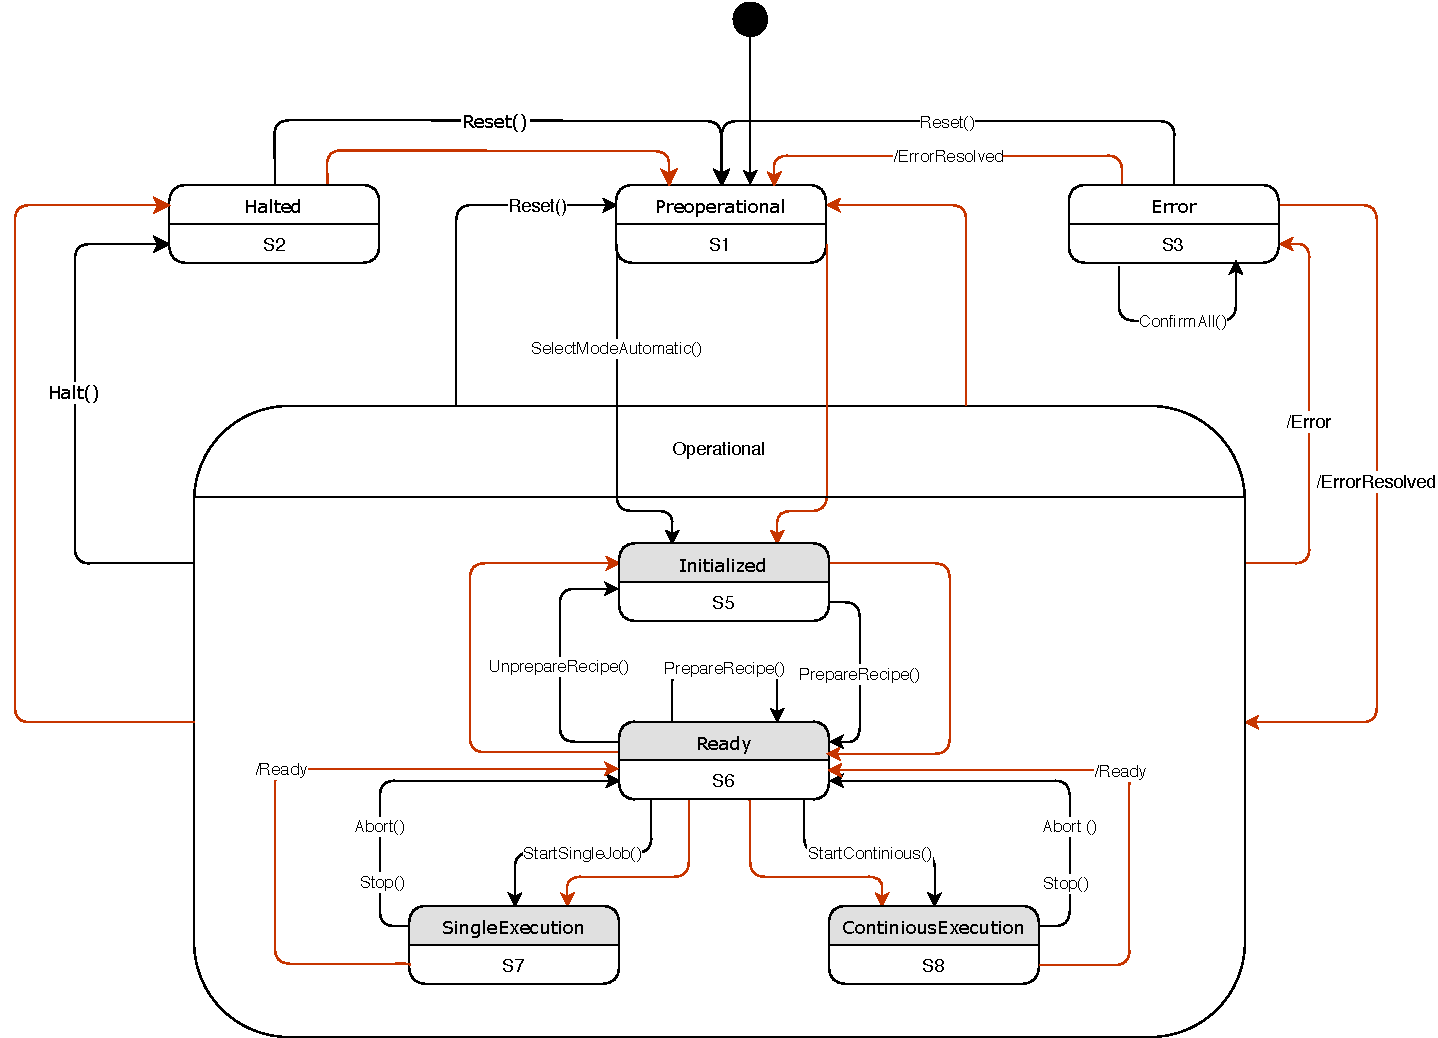
\includegraphics[width=\textwidth]{img/OPCUAVisionVisionAutomaticModeStateMachineStates.pdf}
    \caption[OPC UA Vision state machine in automatic operation mode]{OPC UA Vision state machine in automatic operation mode. Red Lines indicate automatic transitions induced by the vision system with optional effects prefixed with a slash. Black lines indicate method induced transitions with the method name as trigger. The black circle is the entry point of the state machine. All of the states can have optional sub-state machines. States marked in grey are substates.\cite{VDMA2018OPCSpecification}}
    \label{fig:OPCStateMachineAutomatic}
\end{figure}

The information model formally describes all datasets, types, methods, address- and namespaces. See fig. \ref{fig:OPCInfoModelOverview} for an overview and \ref{fig:OPCInfoModelNotation} for an explanation of the notation. The StartSingleJob method (not depicted in the overview) for example triggers transisition from state Ready to SingleExecution in \ref{fig:OPCStateMachineAutomatic}. Its signature consists of following parameters:

\begin{tabbing}
    space \= space \= spacespacespace \= spacespacespacespace \= spacespacespace \kill
    \>  StartSingleJob(\\
    \>  \>  (in)	 \> 	String          \> MeasId\\
    \>  \>  (in)	 \> 	String          \> PartId\\
    \>  \>  (in)	 \> 	RecipeIdType    \> RecipeId\\
    \>  \>  (in)	 \> 	ProductIdType   \> ProductId\\
    \>  \>  (out)	 \> 	String          \> JobId\\
    \>  \>  (out)	 \> 	Int32           \> Error); 
\end{tabbing}

\begin{figure}
    \centering
    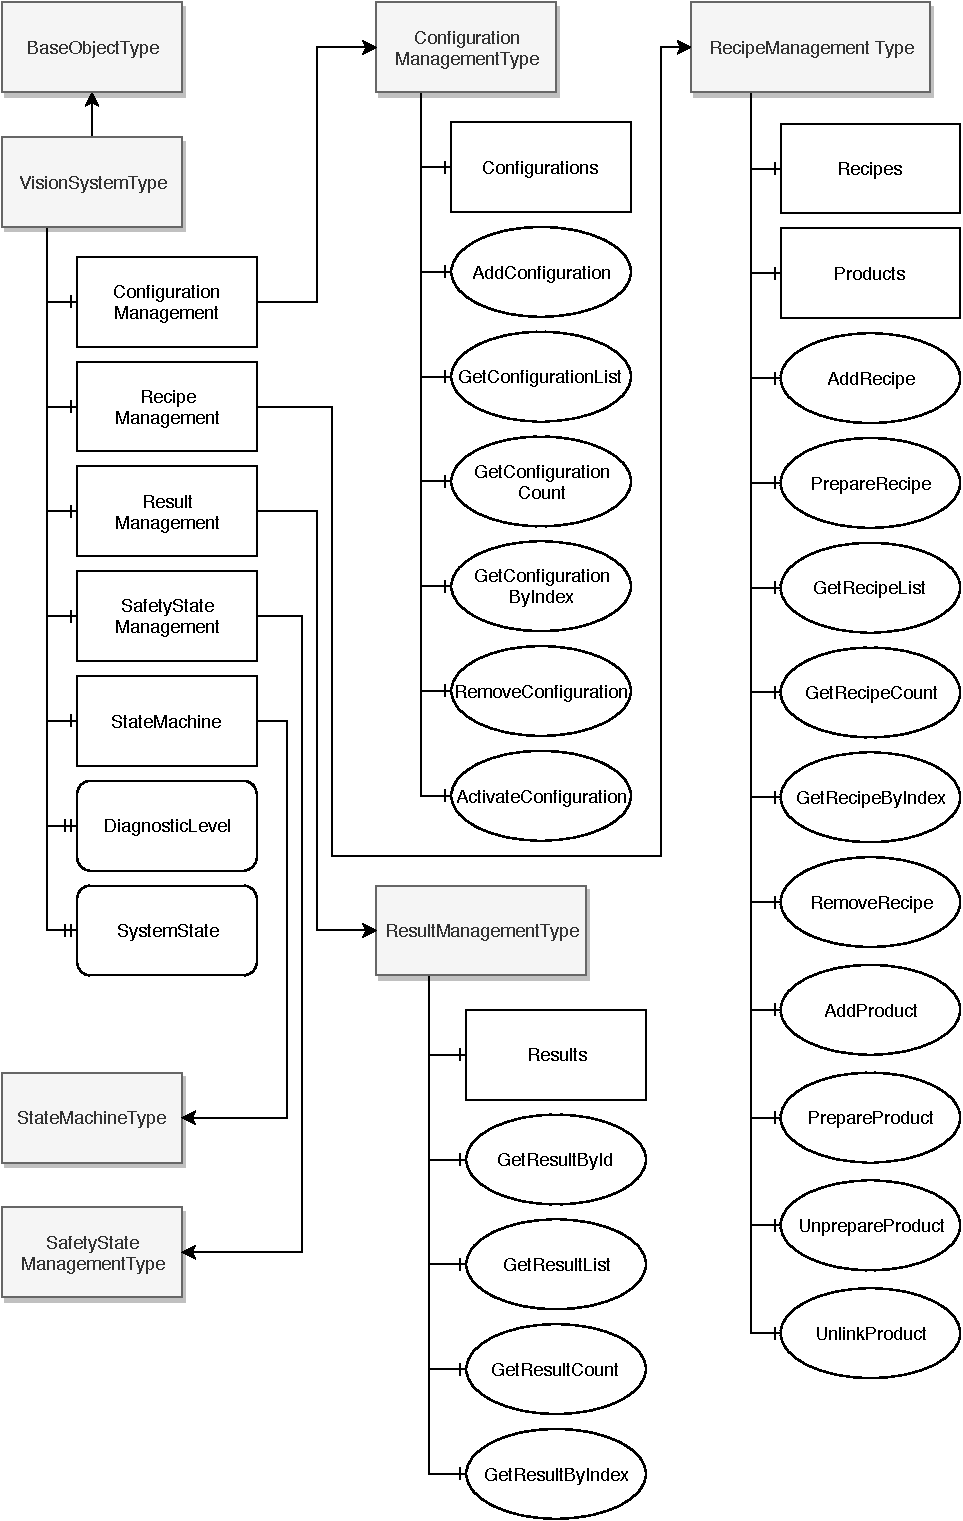
\includegraphics[height=0.9\textheight]{img/OPCUAVisionInformationModelOverview.pdf}
    \caption[OPC UA Vision Information Model Overview]{OPC UA Vision Information Model Overview. See fig. \ref{fig:OPCInfoModelNotation} for a description of the notation.\cite{VDMA2018OPCSpecification}}
    \label{fig:OPCInfoModelOverview}
\end{figure}

\begin{figure}[ht]
    \centering
    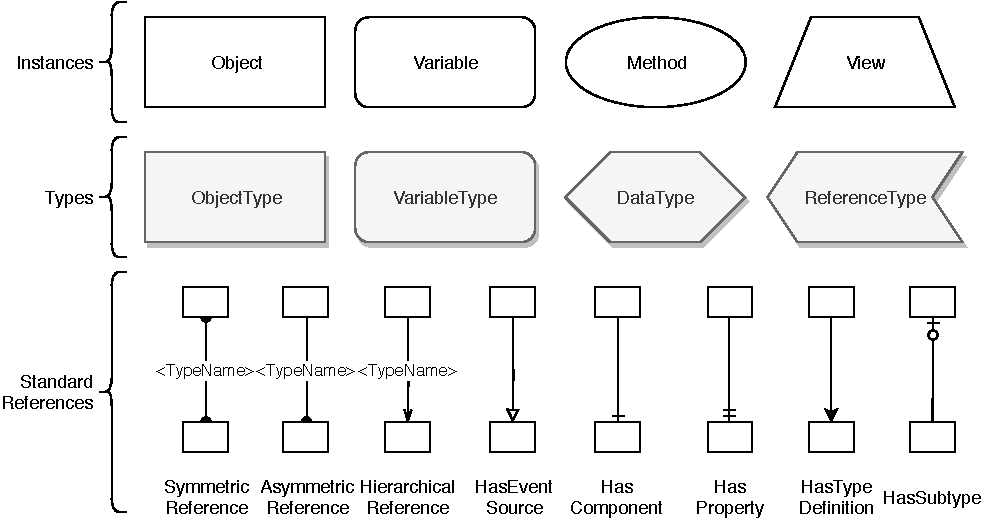
\includegraphics[width=0.8\textwidth]{img/OPCUAVisionInformationModelNotation.pdf}
    \caption[OPC UA Vision Information Model Notation]{OPC UA Vision Information Model Notation.\cite{VDMA2018OPCSpecification}}
    \label{fig:OPCInfoModelNotation}
\end{figure}

The generated OD services should adhere to the OPC UA Vision companion specification. 

To enable exchange with OPC UA servers without the use of an OPC UA stack (enabling
greater interoperability with OPC UA), a holistic translation must translate both structural
and foundational aspects of OPC UA. This means that translation must bypass OPC UA
transport protocols, secure channel management, serialization and OPC UA services - all
in a way that avoids semantic dependencies and preserves translation transparency.

OPC echtzeit praktisch! TSN
\section{Service Generation}
\subsection{Object Detection Method Integration}

\begin{figure}[ht]
    \centering
    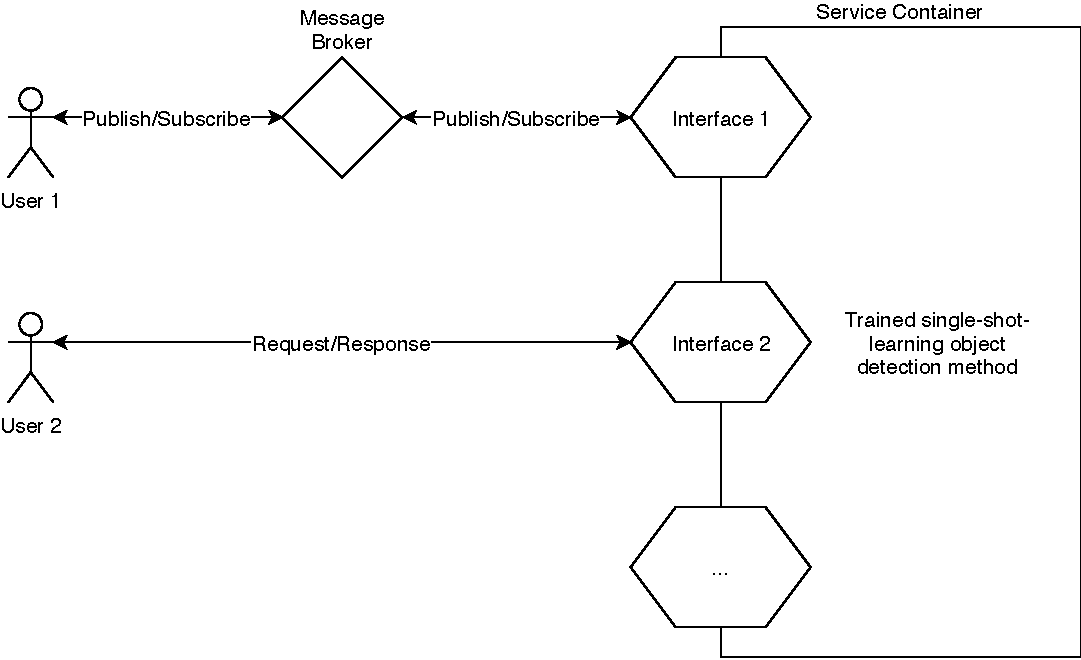
\includegraphics[width=0.8\textwidth]{img/ServiceArchitecture.pdf}
    \caption{Service Interface Architecture.}
    \label{fig:ServiceInterArchit}
\end{figure}

\begin{figure}[ht]
    \centering
    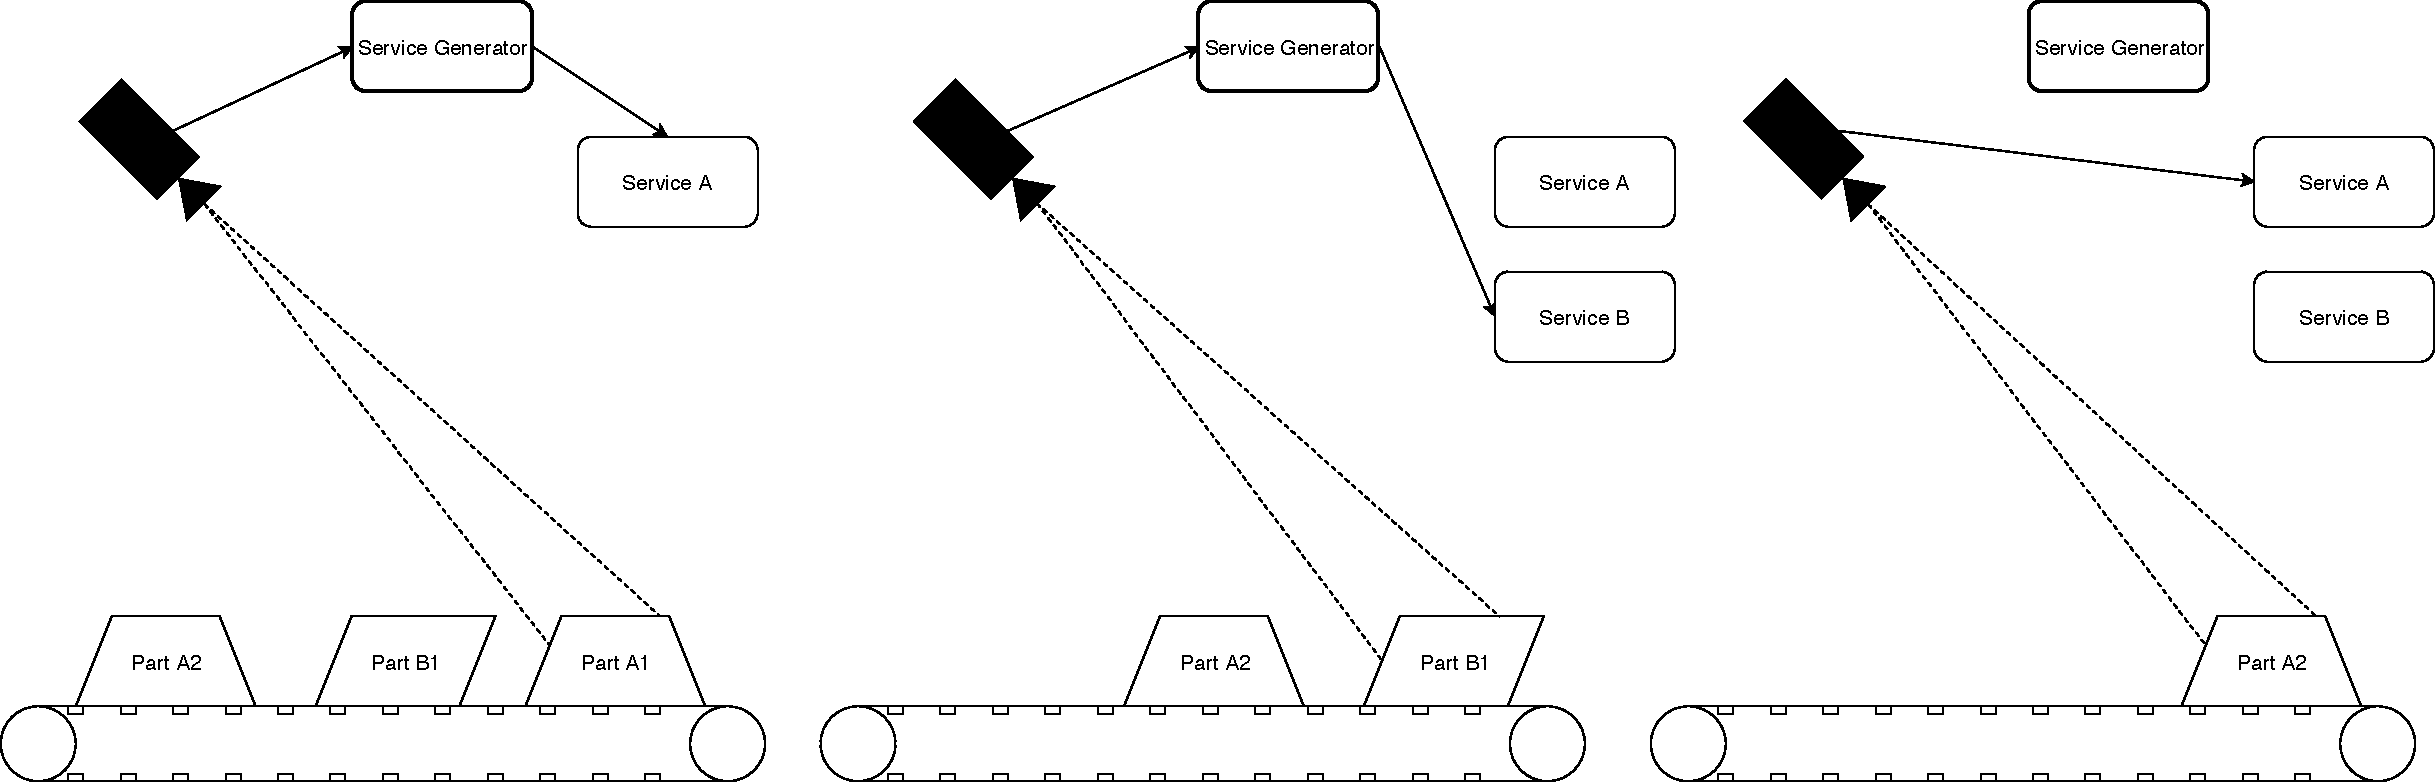
\includegraphics[width=\textwidth]{img/ServiceGenerationExample.pdf}
    \caption{Service generation example in industrial context.}
    \label{fig:ServiceGenExa}
\end{figure}

\subsection{Interface Definition and Protocol Adapters}
For client usability reasons it is beneficial if a service is addressable via several protocols. For example a service using GRPC based on http/2 might want to interact with older web clients which use REST based on http/1.1. IoT devices sometimes only support lightweight publish-subscribe protocols such as MQTT. 

This is also the main issue about gateway middleware, as established in the related
works-section. Because they lack transparency, there is a heavy leakage of endpoint semantics present, which often forces the consumer to understand both the gateway interface
and the endpoint interface. As this creates a semantic dependency, interoperability solutions such as gateway middleware only tend to move the problem rather than solve it.

\begin{table}[]
    \centering
    \begin{tabular}{|c|cccc|}
    \hline
         \diagbox[]{from}{to} & OPC UA & GRPC & REST & MQTT\\\hline
         OPC UA &  \\
         GRPC & \\\hline
         
    \end{tabular}
    \caption{MT translation}
    \label{tab:protoAdptr}
\end{table}

\section{Interoparibility Layers}
siehe Integration of OPC UA with IIoT Protocols chapter 3.1.3

\section{Evaluation Parameters}
As opposed to monolithic applications SOAs are highly agile and easily integrated into distributed systems. This hypothesis has to be supported by qualitative and quantitative test results. An example for a qualitative test would be a test center where the same OD algorithm has to be integrated into a SOA and a monolithic application. The integration should be executed by several equally skilled groups of which one half start with the SOA and the other with the monolithic application. 
Quelle mit Evaluierfragen heranziehen.
Quantitative parameters could be the size of the service containers, the CPU and RAM load they utilize. The usability of the service is also of high impartance, e.g. the number of protocols that the interface offers, the documentation of the interface etc. 

\section{ODS Design and Implementation Possibilities}
\label{sec:concecptOverview}
ODS should be capable of coping with dynamically changing OD algorithms and base protocols. To achieve this, five parameters are relevant: semantic, MT, MT adapter, deployment as and deployment in. Several configurations for each of these parameters are possible. In composition with an ODM, they form a ODS. See \ref{tab:concept} for a graphical representation.\\

% \begin{table}[h]
%     \begin{center}
%       \begin{minipage}{\textwidth}
%         \captionof{table}{Morphological box of the design possibilities of an ODS. Parameters are marked bold in the first column. Every parameter has possible configurations. A combination of configurations composes one concept, marked as colored lines.}\label{tab:concept} 
%         \begin{tikzpicture}[
%             very thick,
%             nodes={inner sep=\tabcolsep}
%           ]
%           \matrix[
%               matrix of nodes,
%               inner sep=0pt,
%               row sep=\zeilenabstand
%             ](m){
%               \grafik{\textbf{Semantic}}{}
%                 &\grafik{existing standard}{}
%                 &\grafik{self designed}{}\\
%               \grafik{\textbf{Interface Architecture}}{}
%                 &\grafik{Client/Server}{}
%                 &\grafik{Publish/Subscribe}{}\\
%               \grafik{\textbf{Deployment as}}{}
%                 &\grafik{Container}{}
%                 &\grafik{VM}{}
%                 &\grafik{}{}\\
%               \grafik{\textbf{Deployment in}}{}
%                 &\grafik{Cloud}{}
%                 &\grafik{Edge}{}
%                 &\grafik{VS}{}
%                 &\grafik{}{}\\
%               &{}&{}&{}&{}\\
%             };
    
%     % Tabellenlinien
    
%             \draw[line width=\heavyrulewidth]([yshift={-\aboverulesep-\zeilenabstand}]m.north west)
%                 --([yshift={-\aboverulesep-\zeilenabstand}]m.north east)
%               ([yshift={-\aboverulesep-\zeilenabstand}]m.south west)
%                 --([yshift={-\aboverulesep-\zeilenabstand}]m.south east);
%     % Verbindungslinien
%             \verbindungslinie{red}{m-1-4}{m-2-3,m-3-4,m-4-3,m-5-2,m-6-2}
%             \verbindungslinie{blue}{m-1-2}{m-2-2,m-4-2,m-5-4,m-6-4}
%             \foreach \f/\p/\t in {red/m-6-2/Non-Industrial,blue/m-6-4/Industrial}
%               \node[\f,below,font=\bfseries]at(\p){\t};
%         \end{tikzpicture}
%       \end{minipage}
%     \end{center}
% \end{table}%


% \begin{table}[h]
%     \begin{center}
%       \begin{minipage}{\textwidth}
%         \captionof{table}{Morphological box of the implementation possibilities of an ODS. Parameters are marked bold in the first column. Every parameter has possible configurations. A combination of configurations composes one concept, marked as colored lines.}\label{tab:concept} 
%         \begin{tikzpicture}[
%             very thick,
%             nodes={inner sep=\tabcolsep}
%           ]
%           \matrix[
%               matrix of nodes,
%               inner sep=0pt,
%               row sep=\zeilenabstand
%             ](m){
%               \grafik{\textbf{Semantic}}{}
%                 &\grafik{OPC UA Vision}{}
%                 &\grafik{GCV RPC API}{}
%                 &\grafik{ODM}{}
%                 &\grafik{self designed}{}\\
%               \grafik{\textbf{Base MT}}{}
%                 &\grafik{OPC UA}{}
%                 &\grafik{GRPC}{}
%                 &\grafik{REST}{}
%                 &\grafik{MQTT}{}\\
%               \grafik{\textbf{MT Adapter}}{}
%                 &\grafik{OPC UA}{}
%                 &\grafik{GRPC}{}
%                 &\grafik{REST}{}
%                 &\grafik{MQTT}{}\\
%               \grafik{\textbf{Deployment as}}{}
%                 &\grafik{Docker}{}
%                 &\grafik{Heroku}{}
%                 &\grafik{VM}{}
%                 &\grafik{}{}\\
%               \grafik{\textbf{Deployment in}}{}
%                 &\grafik{Cloud}{}
%                 &\grafik{Edge}{}
%                 &\grafik{VS}{}
%                 &\grafik{}{}\\
%               &{}&{}&{}&{}\\
%             };
    
%     % Tabellenlinien
    
%             \draw[line width=\heavyrulewidth]([yshift={-\aboverulesep-\zeilenabstand}]m.north west)
%                 --([yshift={-\aboverulesep-\zeilenabstand}]m.north east)
%               ([yshift={-\aboverulesep-\zeilenabstand}]m.south west)
%                 --([yshift={-\aboverulesep-\zeilenabstand}]m.south east);
%     % Verbindungslinien
%             \verbindungslinie{red}{m-1-4}{m-2-3,m-3-4,m-4-3,m-5-2,m-6-2}
%             \verbindungslinie{blue}{m-1-2}{m-2-2,m-4-2,m-5-4,m-6-4}
%             \foreach \f/\p/\t in {red/m-6-2/Non-Industrial,blue/m-6-4/Industrial}
%               \node[\f,below,font=\bfseries]at(\p){\t};
%         \end{tikzpicture}
%       \end{minipage}
%     \end{center}
% \end{table}%



Semantic defines the interface of the service. It handles the payload of the communication between server and client. That is depending on messaging technology, service definition of methods, return types and resources. OPC UA Vision \cite{VDMA2018OPCSpecification} and GCV RPC API \cite{Lastvisited2018-11-272018CloudGRPC} are two publicly available standards for ODS. In general, resorting to public standards is a good habit due to the already existing user base, detailed documentation, constant development and thorough testing. In contrast to that one could design the semantic for a service interface on his own with the advantage of freedom over all design decisions. However, this would mean a constant update of design work when adapting to new protocols or ODM, which is tedious and does not outweigh the advantages of public standards. When comparing OPC UA Vision and GCV RPC API one can see that the former is meant to be an abstract standard for all kinds of vision systems, the latter is tailored for the GCV service. Through abstraction the former is more durable than the latter. Also, OPC UA Vision is maintained by the OPC foundation and thus focuses on industrial applications. Another way of defining the service would be copying the method signatures and return types of the ODM. This would mean a changing interface towards the client with every new ODM, which is not eligible in the context of the fast-changing world of underlying ODM of the service. Instead, the semantic translation between ODM and service methods should be hidden. \\

MT defines how data is transported between entities. This includes base protocols, security designs, encoding and data transfer insurance. Note that since February 6, 2018 OPC UA offers the possibility to send its data via MQTT as specified in part 14 of the OPC UA specification, so you could "include" MQTT into OPC UA. However, MQTT can be used as a standalone MT, offering less features especially concerning information modeling, but with the advantage of creating less overhead. Also, the OPC UA can utilize HTTPS for transport, however not in a RESTful manner. \cite{Ronnholm2018IntegrationTranslator} This is due to a lacking adressing scheme. RESTful HTTP is centered around abstract resources that can be identified by a URL. Any body of data may therefore be manipulated independently of any intermediary application logic. This is not the case with HTTP in OPC UA. In addition, HTTP is deeply embedded into the communication stack and can therefore not be understood by an unrelated third party. Ronnholm introduces a possible adapter in his thesis. \cite{Ronnholm2018IntegrationTranslator}

The environment (e.g. industrial or home automation) of the service has an effect on the MT. Especially for industrial environments a connection to OT is highly beneficial for real time applications. 

For convenience, one or more adapter can be offered towards the client or other ODS. \\

Deployment as Heroku container is possible, although dependent on the Heroku platform thus dependent on cloud deployment. For some use cases, especially those that require low latency, an edge deployment is more applicable. \\

There are many more implementation possibilities such as database integration, orchestration vs. choreography, continuous deployment and so forth. These aspects are not remarked in the concept phase of thesis as they are considered implementation specific.

The following section introduce a possible concept for an ODS in an industrial environment.